%!TEX root = ../dynamics.tex
\section{The Evolution of Amazon MTurk: 2009 to 2014}\label{sec:stats}


\subsection{Crowdsourcing Platform Dataset}
\label{sec:tracker}
Over the past five years, we have periodically collected data about HITs being published on \amt{}.
Real-time data that we collect about the platform is available at \url{http://mturk-tracker.com/}. In this work we consider hourly aggregated data that includes the available HIT batches and their metadata (tittle, description, rewards, required qualifications, etc.), in addition to their progress overtime, that is, the temporal variation of HITs available. In fact, one of the main metrics that we investigate (see Section \ref{sec:throughput}) is the throughput of a batch, i.e.,  how many HITs  get completed between two observations. Note that our data collection system acts  as a periodic observer and does not reflect fine grained information (e.g., variations at each second). We believe however that the data captures enough information to perform long term trend analysis to understand the dynamics and interactions within crowdsourcing platforms.\\

\gd{add exact total number of HITs}

\subsection{A Data-driven Analysis of Platform Evolution}
First, we identify some trends obtained from aggregated information over time, keywords or countries associated with published HITs.  Each of the following analyses is also available as an interactive visualization over the historical data on \url{http://xi-lab.github.io/mturk-mrkt/}.
\paragraph{Topics  Over Time}
First we want to understand how different topics have been addressed by means of micro-task crowdsourcing over time.
In order to do such analysis we look at the keywords associated with published HITs. We observe the evolution of keyword popularity and associated reward on \amt{}. 
%plot explanation
Figure \ref{fig:tagEvolution} shows such behavior. Each point in the plot represents a keyword associated to HITs with its frequency (i.e., number of HITs with such keyword) on the x-axis, the average reward in a certain year of HITs with this keyword on the y-axis. The path connecting data points indicates the time evolution, starting in 2009, with one point representing the keyword usage over one year.

% observations
We can observe that the `audio' and `transcription' keywords (i.e., blue and red paths from left to right) have substantially increased in frequency over time being among the most popular keywords in the last two years and are paid more than \$1 on average.
HITs with the `video' tag have also increased in number with a reward that has reached a peak in 2012 and decreased after that.
HITs tagged as `categorization' have been paid constantly in the range of \$0.10-\$0.30 on average, except in 2009 where they were rewarded less than \$0.10 each.
HITs tagged as `tweet' have not increased in number but have been paid more over years reaching \$0.9 on average in 2014: This can be explained by more complex tasks being requested to workers: for example, from sentiment classification to writing a new tweet.

\begin{figure}[ht]
	\centering
		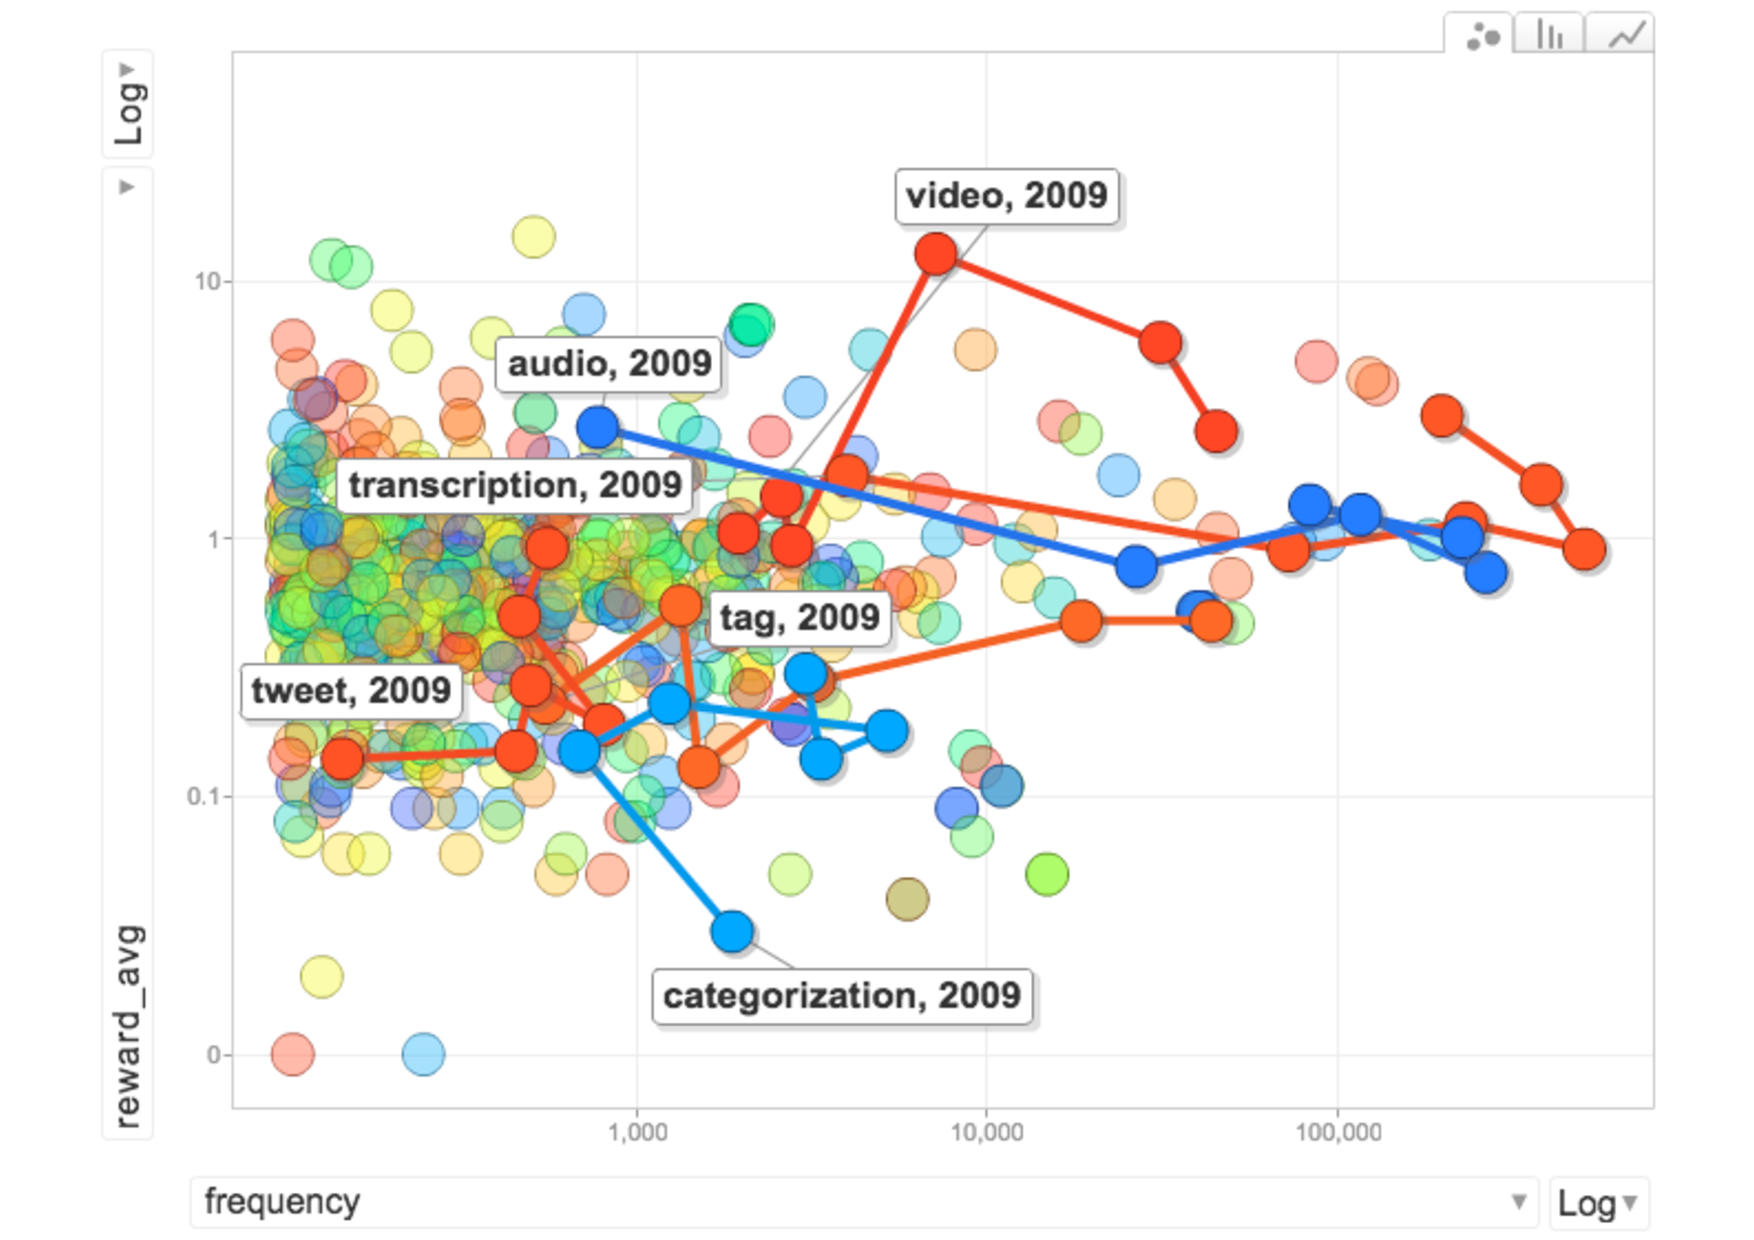
\includegraphics[width=0.5\textwidth]{figures/tagEvolution}
	\caption{The use of keywords to tag HITs with their frequency and reward over time.}
	\label{fig:tagEvolution}
\end{figure}

\paragraph{Preferred Countries by Requesters Over Time}
Figure \ref{fig:country} shows the requirements of requesters with respect to which countries they need workers from. The left part of Figure \ref{fig:country} shows that most HITs are to be completed exclusively by workers located in US, India, or Canada. The right part of Figure \ref{fig:country} shows the evolution over time of the country requirement phenomena.
The plot shows the number of HITs with a certain country requirement (on the y-axis) and its time evolution (on the x-axis) with yearly steps. The size of the data point indicates the total reward associated to those HITs.

We can see that US-only HITs dominate both in terms of number as well as of reward associated to them. 
Interestingly, we notice how over time HITs for workers based in India have been decreasing. This can be explained by \amt restrictions on accepting new workers on the platform.
On the other hand, HITs for workers based in Canada have been increasing over time becoming in 2014 more than those exclusively available to workers based in India.  We also see that the reward associated to them is less as compared to the budget for India-only HITs.
As of 2014, both HITs for workers based in Canada or UK are more numerous that those for workers based in India.
Overall, 88.5\% of the HIT batches that were posted in the considered time period did not require any specific worker location, and 86\% of those who did requested US based workers.
\begin{figure*}[ht]
	\centering
		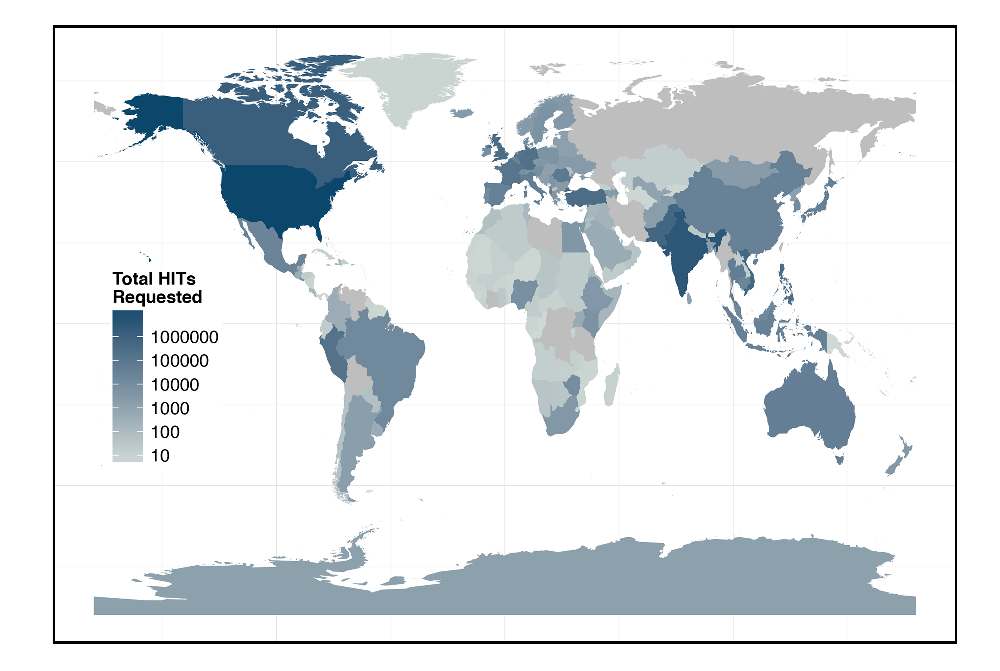
\includegraphics[width=0.43\textwidth]{figures/map}
		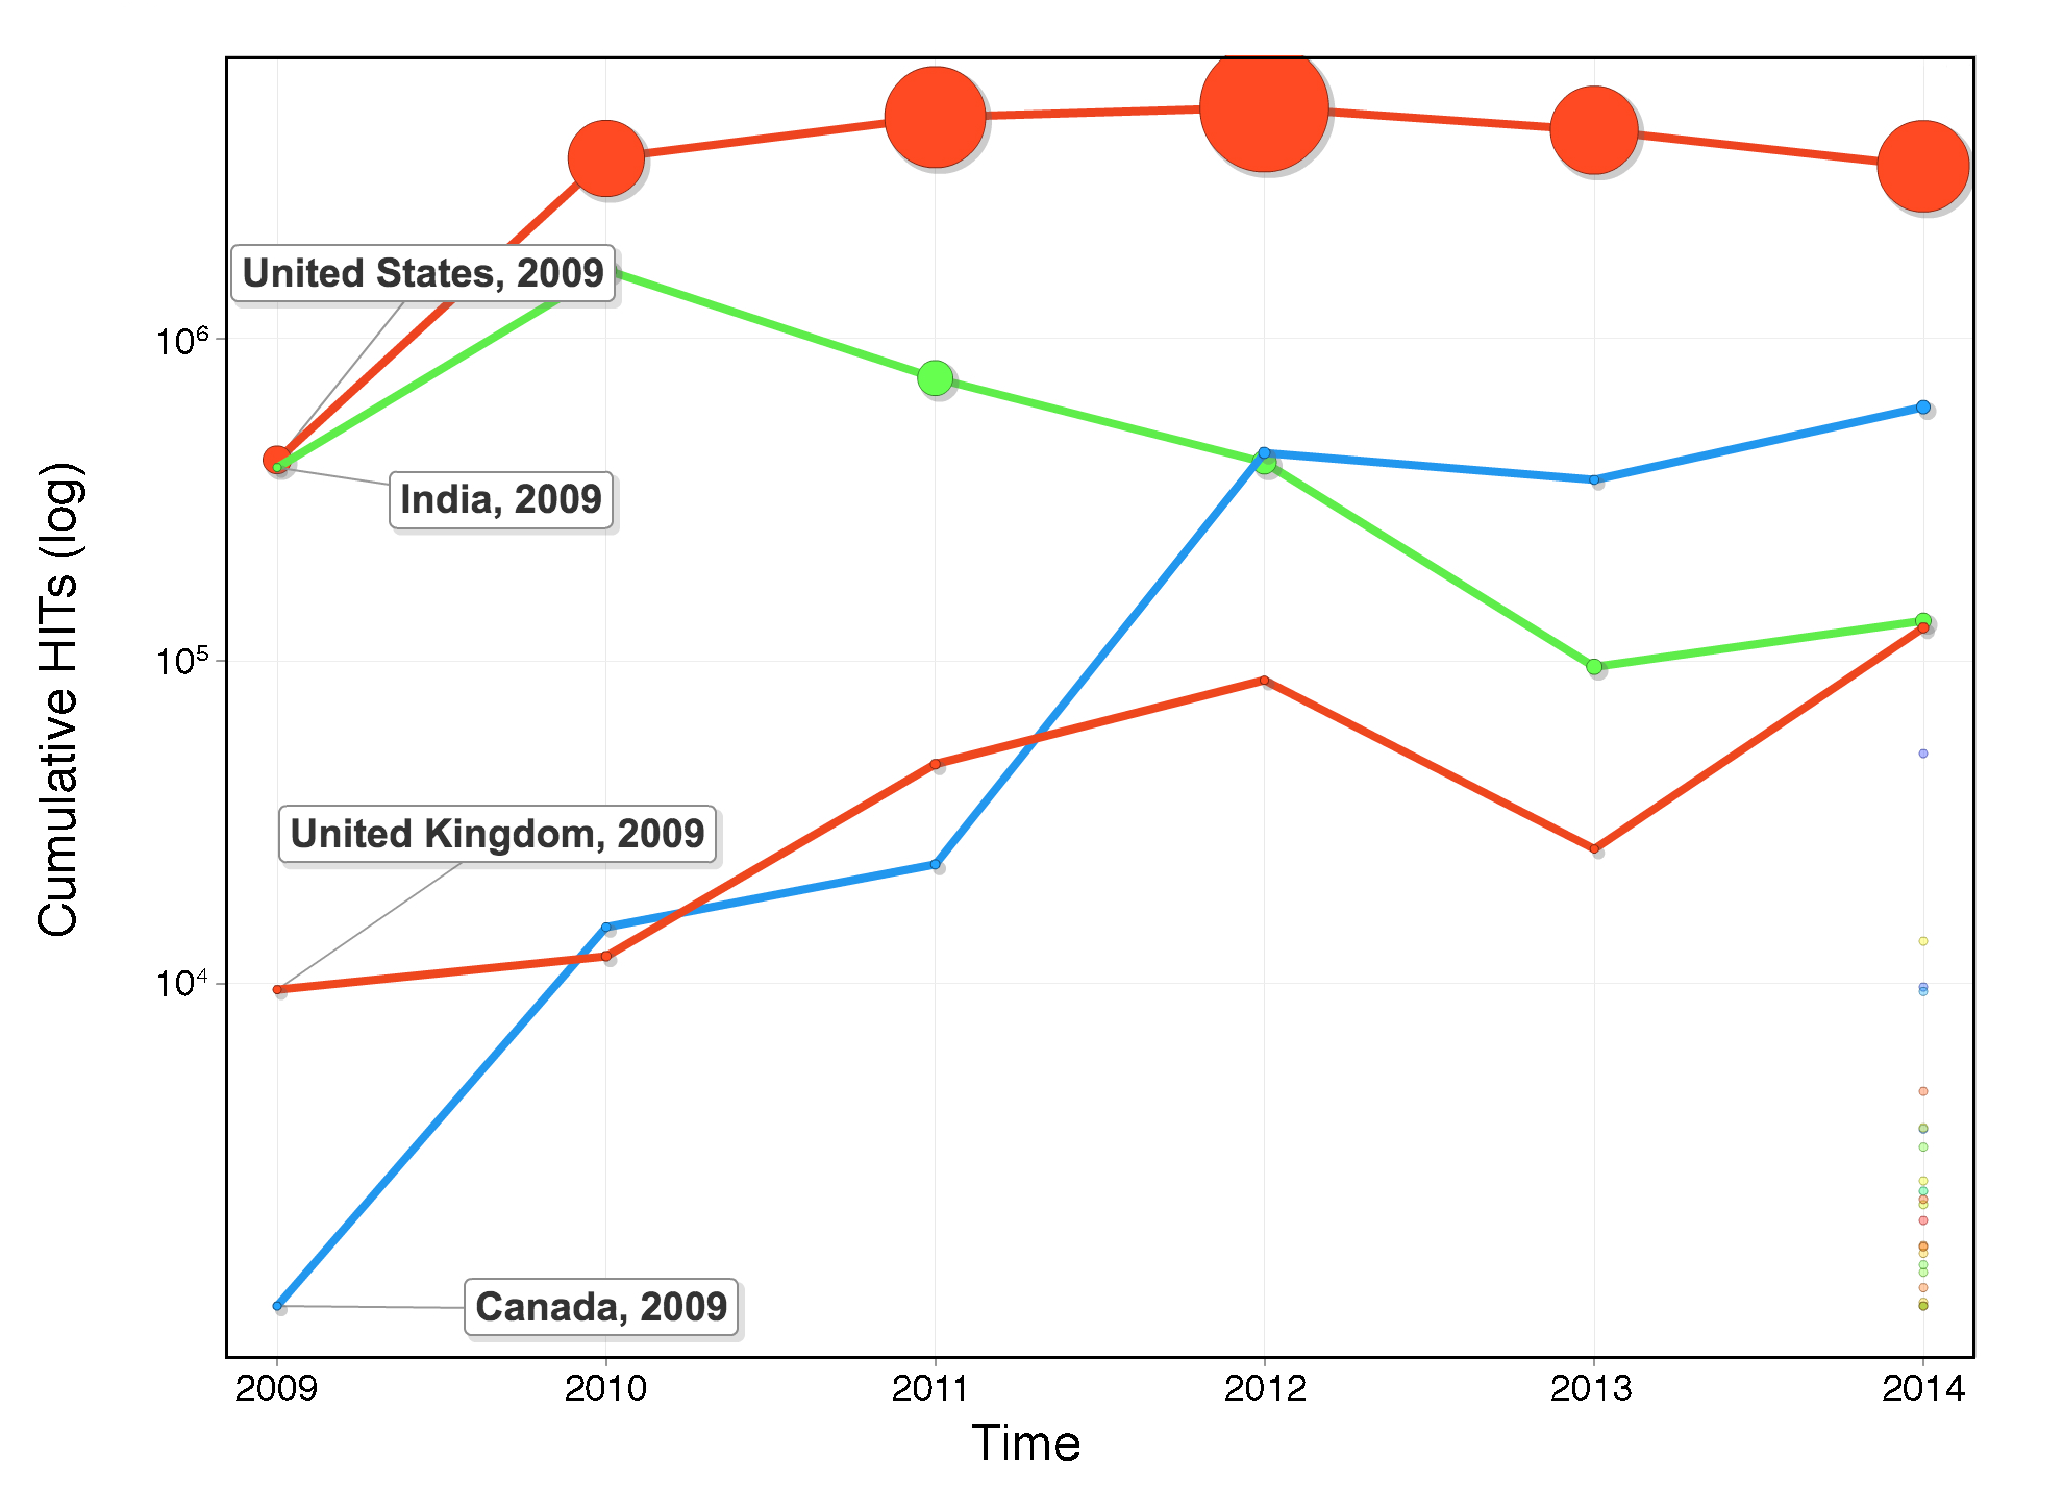
\includegraphics[width=0.43\textwidth]{figures/countriesTime}
	\caption{HITs with specific country requirements. On the left, the countries with most HITs dedicated to them. On the right, the time evolution (x-axis) of country specific HITs with volume (y-axis) and reward information (size of data point).}
	\label{fig:country}
\end{figure*}

Figure \ref{fig:keyword_loc} shows the top keywords attached to HITs restricted to specific locations.
\begin{figure}[ht]
	\centering
		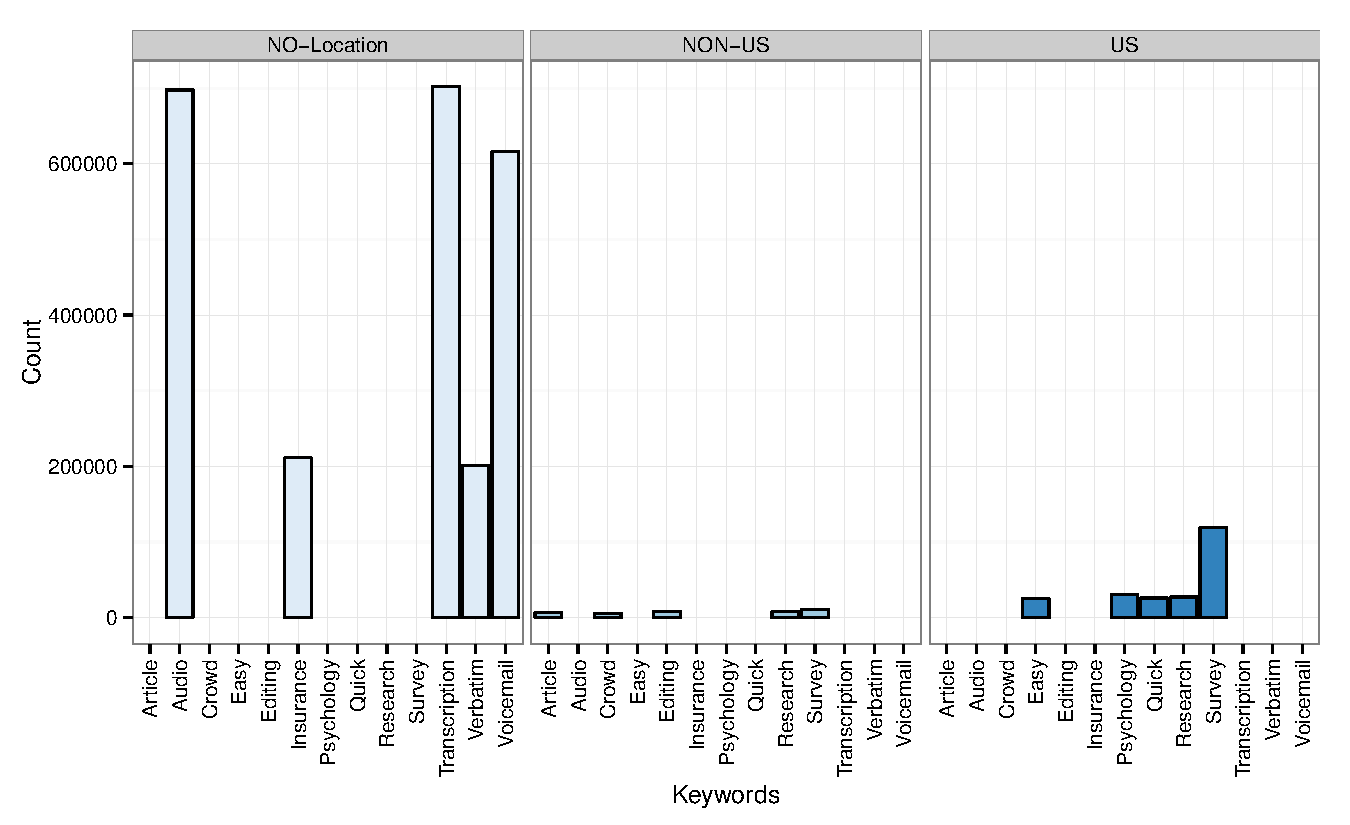
\includegraphics[width=0.5\textwidth]{figures/keywords_location}
	\caption{Keywords for HITs restricted to specific countries.}
	\label{fig:keyword_loc}
\end{figure}
We can see that the most popular keywords (i.e., `audio' and `transcription') do not require country-specific workers. This can be explained by the fact that restricting on workers from a single country for such large amount of HITs would make their completion much slower. We also note that US-only HITs are most commonly tagged with `survey'.

% \subsection{Why Did Certain Requesters Quit?}
% \subsection{Does reputation Improve Throughput?}

\paragraph{HIT Reward Analysis}
Figure \ref{fig:reward_year} shows most frequent rewards assigned to HITs over time\footnote{Data for 2014 has been omitted as not comparable with other year values.}. We can see that while in 2011 the most popular reward was \$0.01, more recently HITs paid \$0.05 are more frequent. This can be explained by both how workers search for HITs on \amt{} and by the \amt{} fee scheme. Requesters now prefer to publish more complex HITs possibly with multiple questions in it and grant an higher reward: This attracts also those workers who are not willing to complete a HIT for a too small pay and reduces the fees paid to \amt{} which are computed also based on the number of HITs published on the platform.

\begin{figure}[ht]
	\centering
		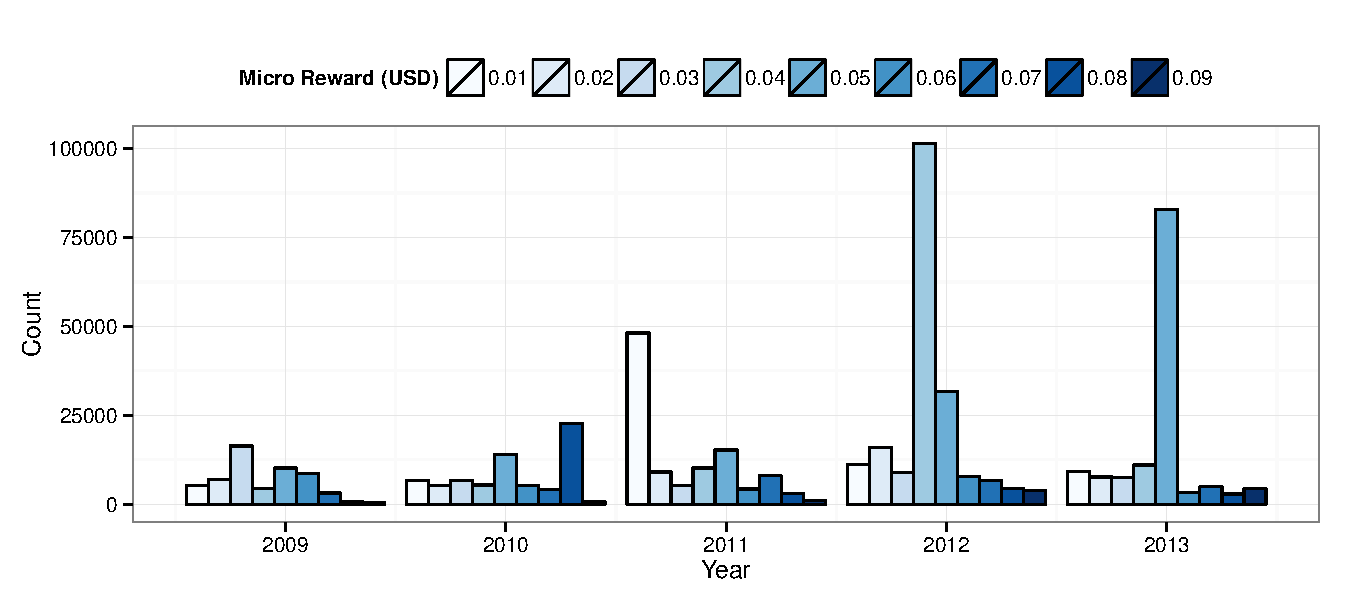
\includegraphics[width=0.5\textwidth]{figures/reward_year}
	\caption{Popularity of HIT reward values over time. \gd{can we add 0.10?}}
	\label{fig:reward_year}
\end{figure}



\paragraph{Requester Analysis}
In order to be sustainable, a crowdsourcing platform needs to retain requesters over time or get new requesters to replace those who do not publish HITs anymore. Figure \ref{fig:requesters_reward} shows the number of new requesters who used \amt{} and the overall number of active requesters at a certain point in time. We can observe an increasing number of active requesters over time and a constant number of new requesters who join the platform (at a rate of 1000/month over the last two years).

\begin{figure}[ht]
	\centering
		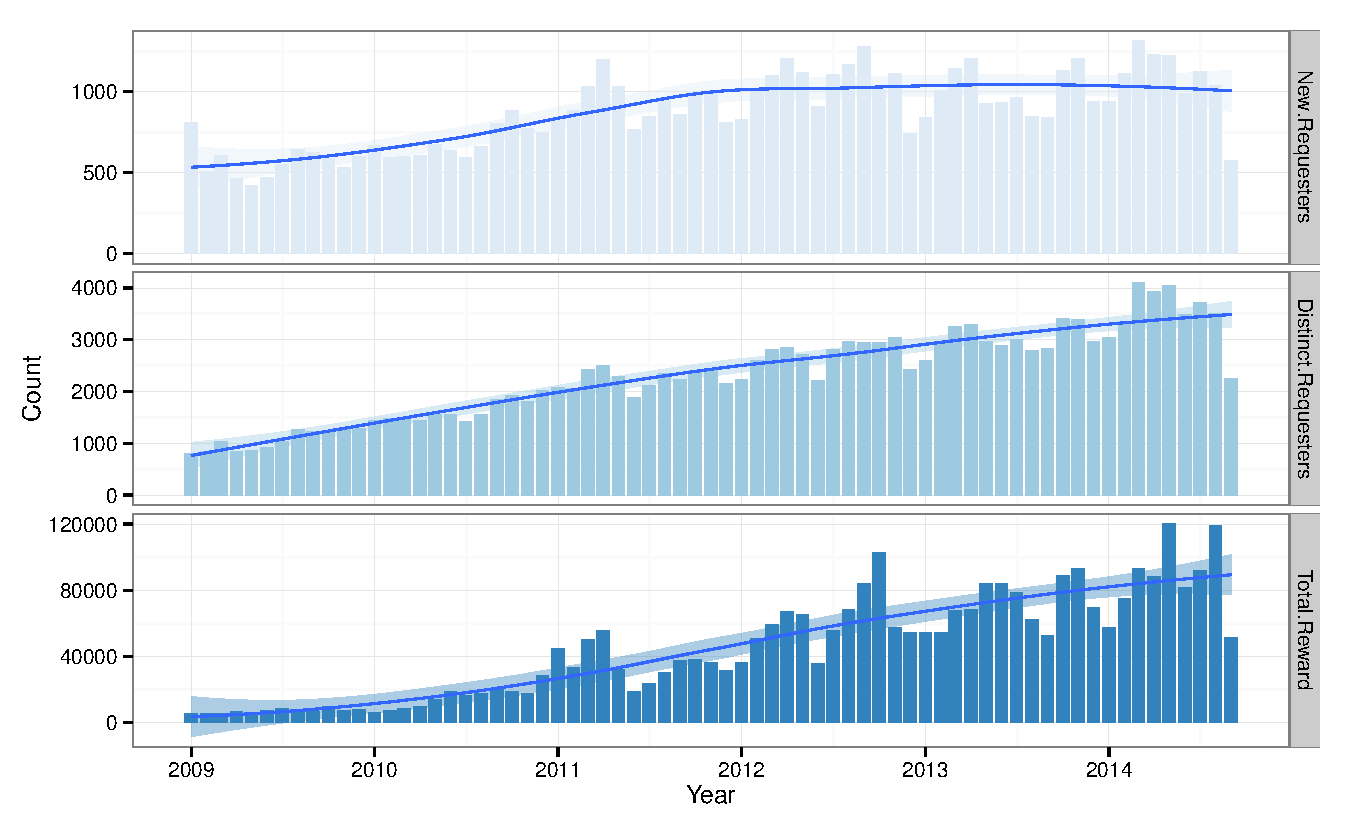
\includegraphics[width=0.5\textwidth]{figures/requesters_reward}
	\caption{Requester activity and total reward on the platform over time. The line over the data shows local polynomial regression fitting \cite{cleveland1992local}.}
	\label{fig:requesters_reward}
\end{figure}

To better understand the financial health of the crowdsourcing platform, it is also interesting to look at the overall amount of rewards for HITs  published on the platform as platform revenues are computed as a  function of  HIT rewards. From the bottom part of Figure \ref{fig:requesters_reward} we can  observe a linear increase in the total reward for HITs on the platform. Interestingly, we can also observe certain seasonality effects over years with October being the month with highest total reward and January or February being the month with minimum total reward.


\paragraph{HIT Batch Size Analysis}
When a lot of data needs to be crowdsourced (e.g., many images to tag), multiple similar HITs are published together. We define a batch of HITs as such set of similar HITs published by a requester at a certain point in time. Figure \ref{fig:batch_size} shows how  batch size has changed over time.
We can see that while, on average, batches have been getting smaller, in 2014 very large batches have appeared on \amt{} indicating a clear business interest and scalability demand from micro-task crowdsourcing.

\begin{figure}[ht]
	\centering
		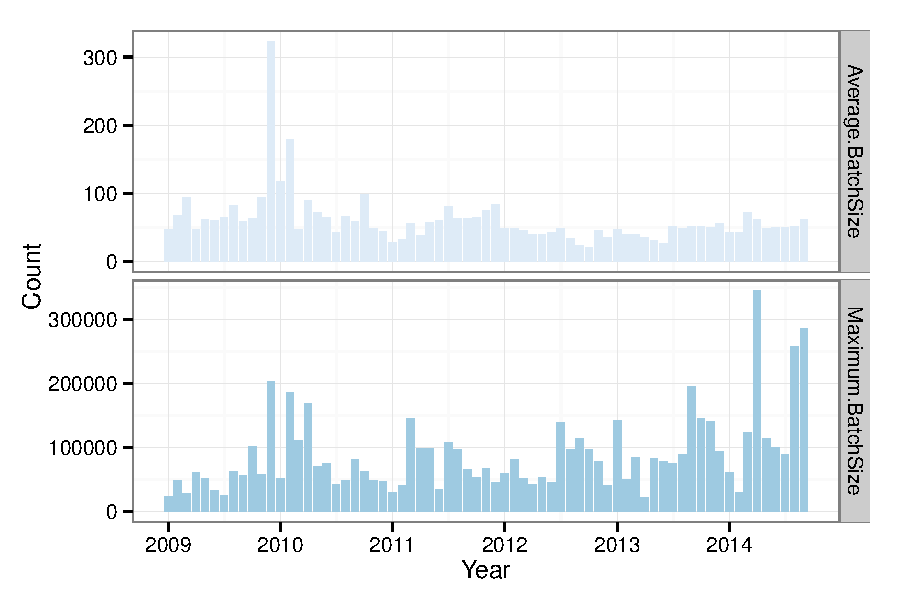
\includegraphics[width=0.5\textwidth]{figures/batch_size}
	\caption{Batch Sizes. The line over the data shows local polynomial regression fitting \cite{cleveland1992local}.}
	\label{fig:batch_size}
\end{figure}


